\graphicspath{{images/generalFigures/}, {images/word_cloud/}}

\begin{frame}[plain]{}
  \begin{beamercolorbox}[wd=\paperwidth,ht=\paperheight]{frametitle}
    \begin{tikzpicture}
      \fill[azulunam, opacity=1] (0, 0) rectangle(100, 100);
      \node [anchor=center] (cloud) at 
        (0.5\paperwidth, 0.5\paperheight)
        {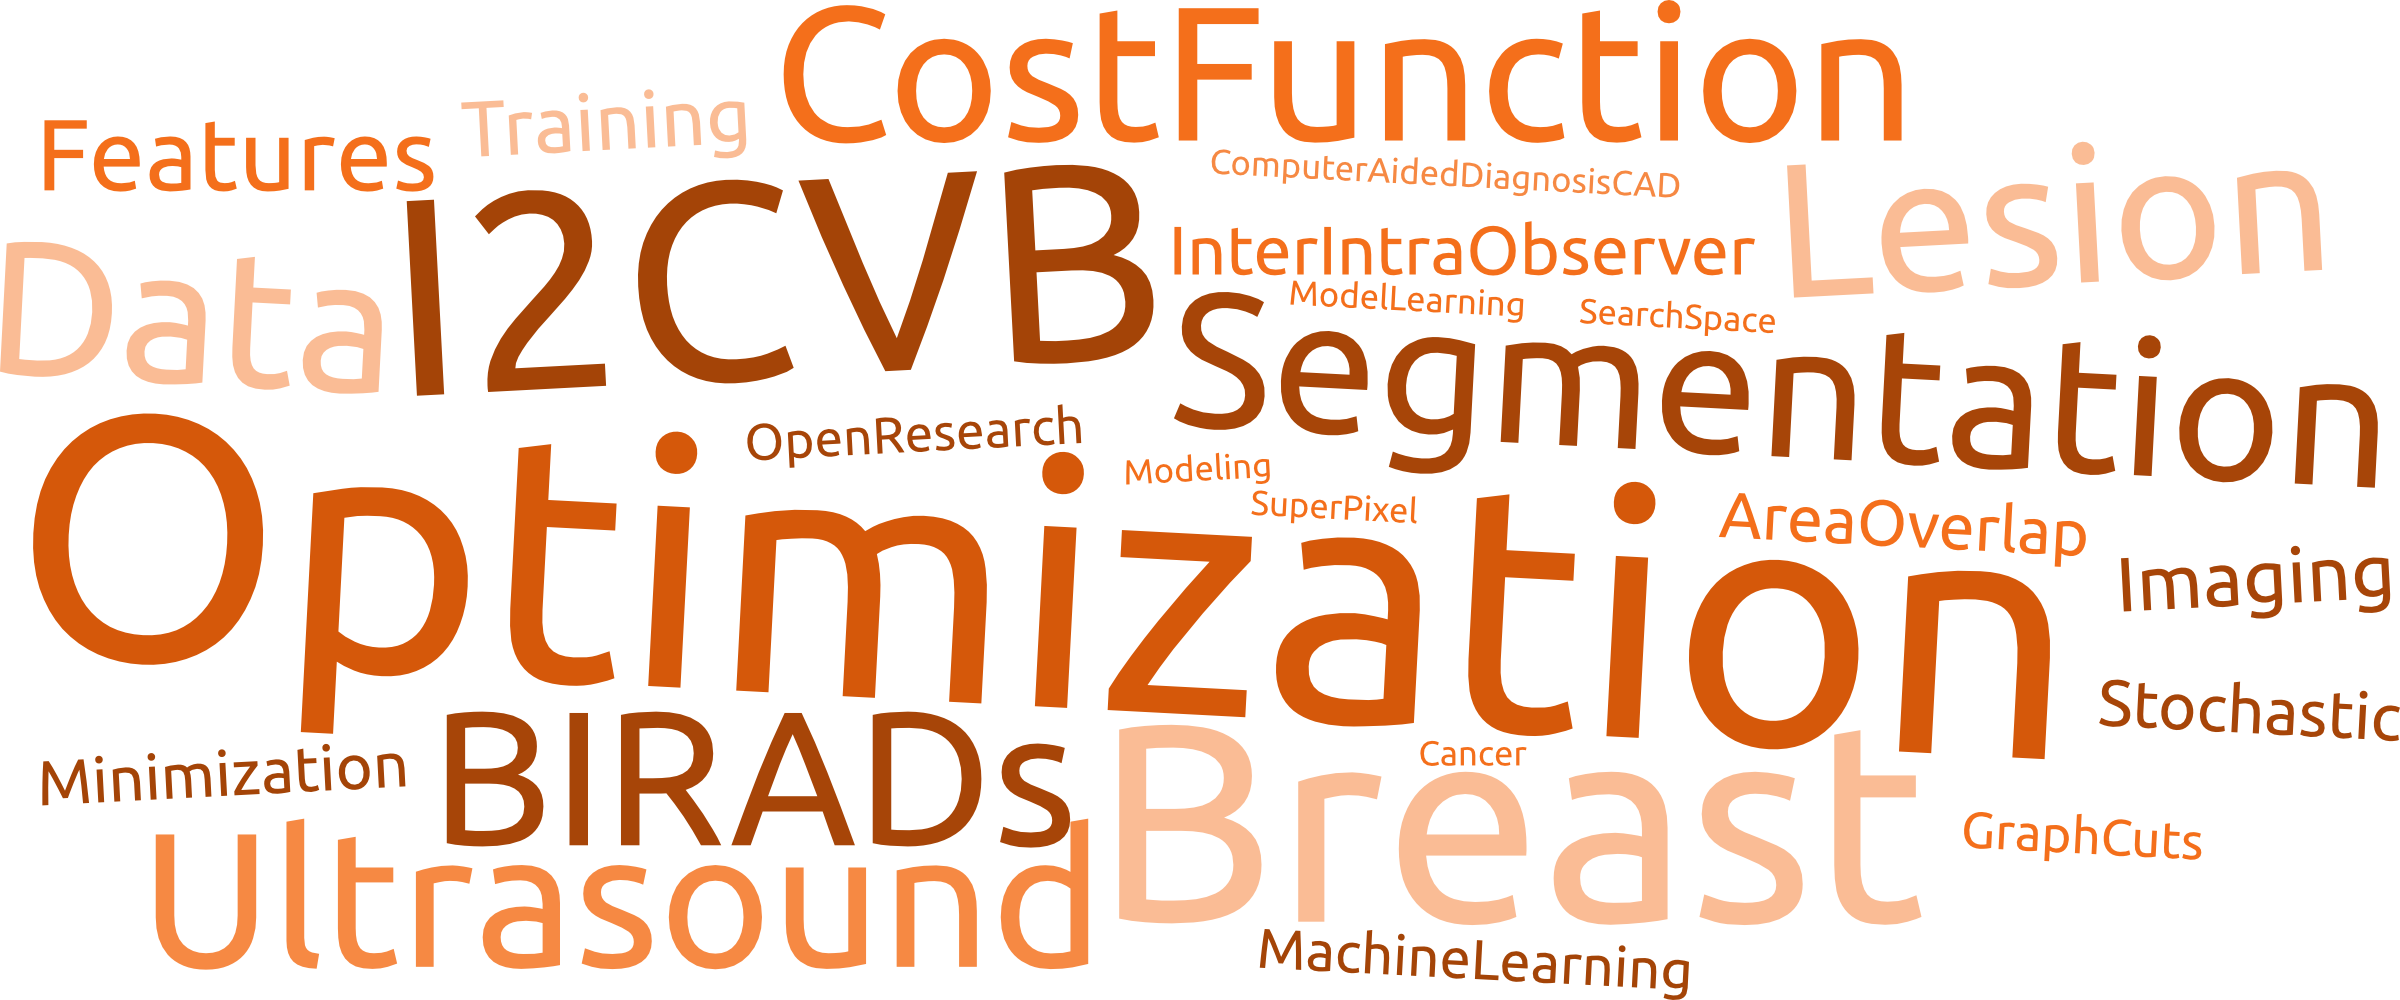
\includegraphics[width=.95\paperwidth]{orange_mix.png}};
    \end{tikzpicture}
  \end{beamercolorbox}
  % 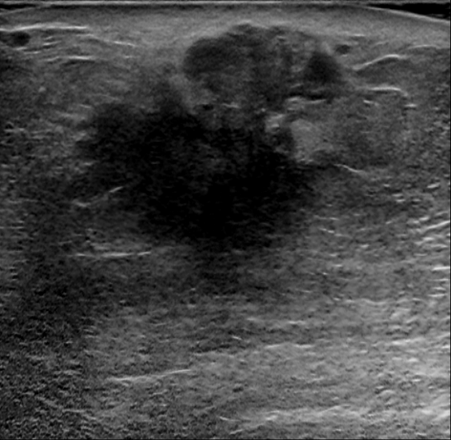
\includegraphics[trim=0 6 0 0,clip,height=.65\textheight]{a110105_094.png}~
\end{frame}


\begin{frame}[plain]{}
  \begin{beamercolorbox}[wd=\paperwidth,ht=\paperheight]{frametitle}
    \begin{tikzpicture}
      \fill[azulunam, opacity=1] (0, 0) rectangle(100, 100);
      \node [anchor=center] (cloud) at 
        (0.5\paperwidth, 0.5\paperheight)
        {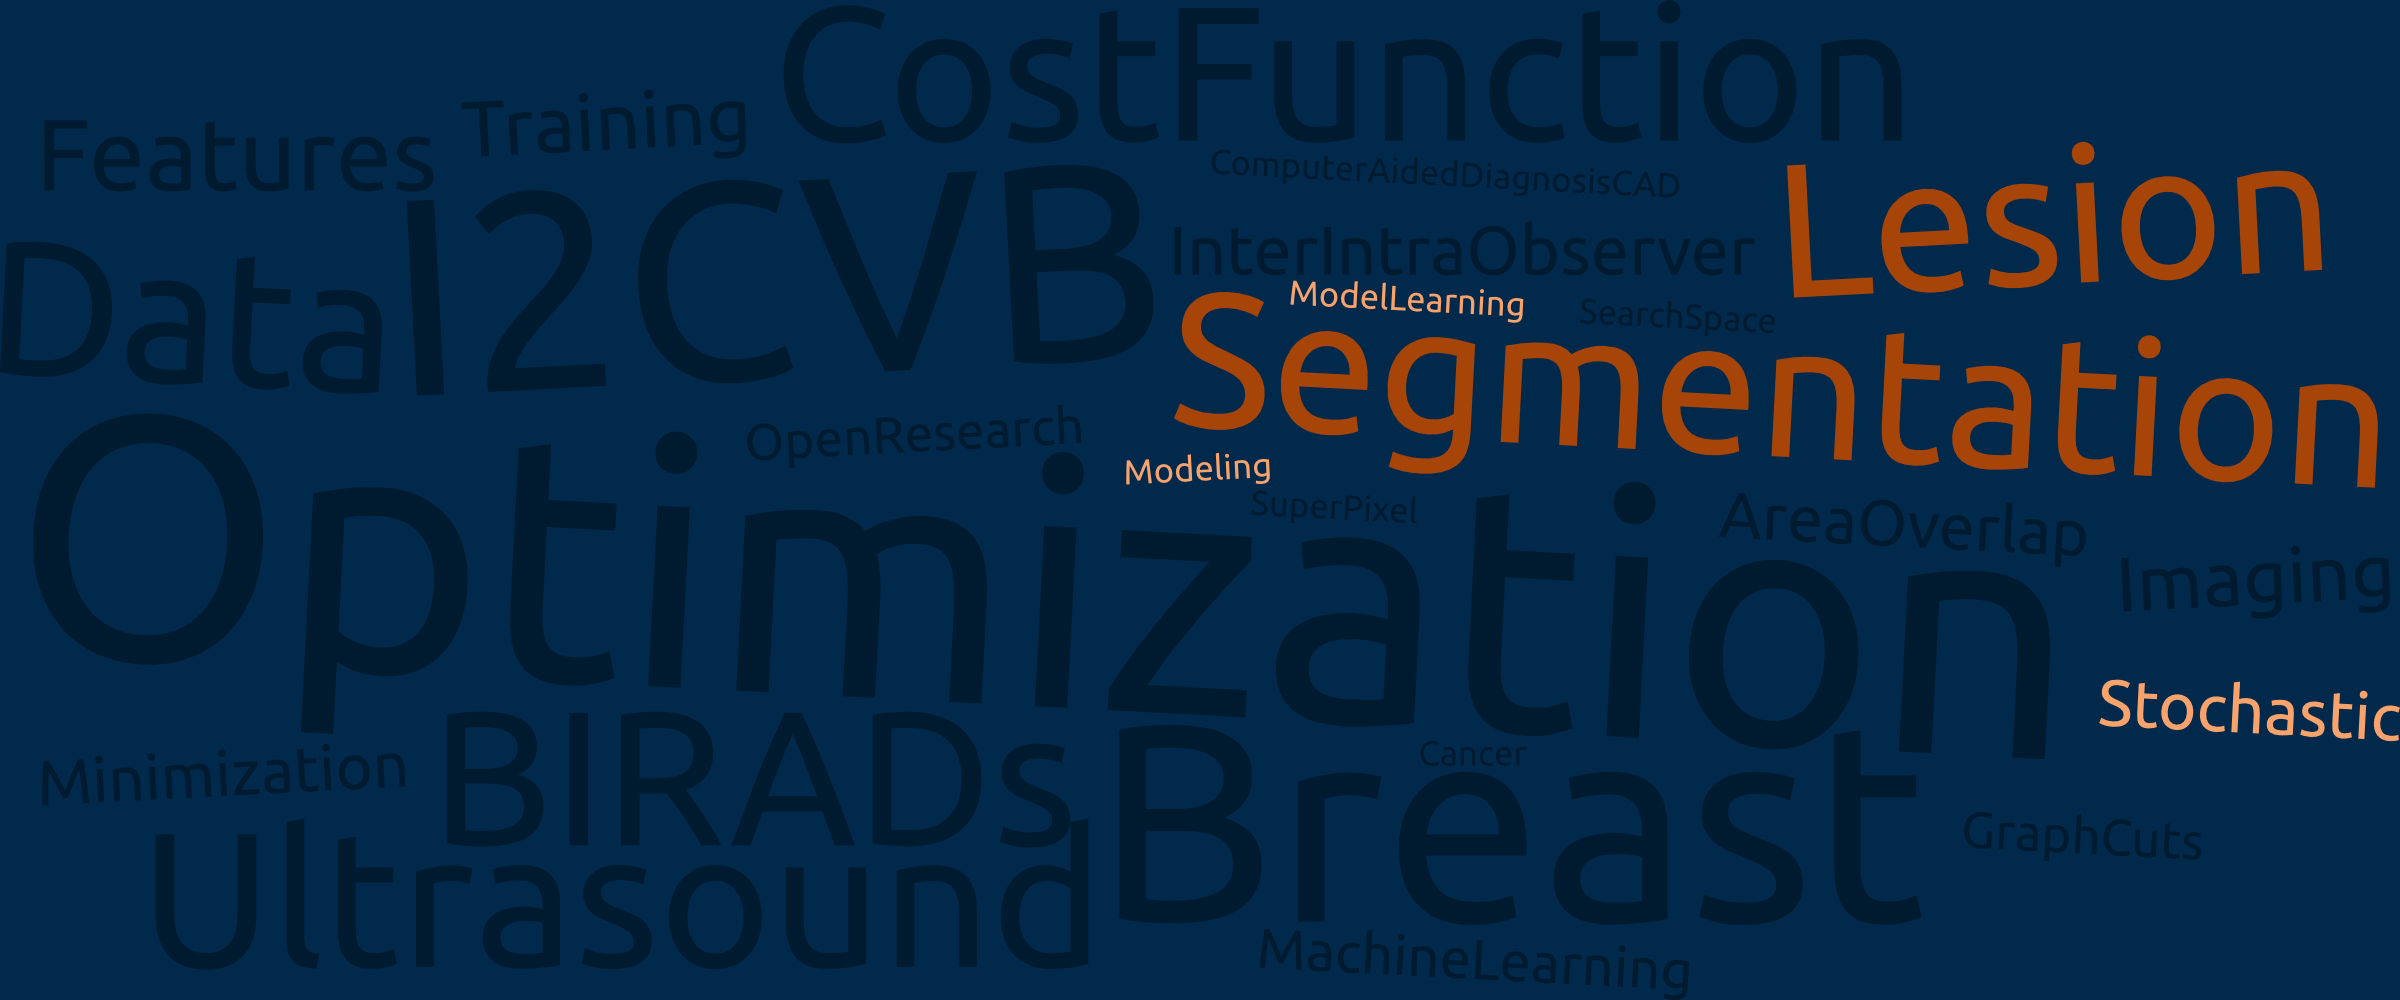
\includegraphics[width=.95\paperwidth]{highlight_prelude.png}};
    \end{tikzpicture}
  \end{beamercolorbox}
  % 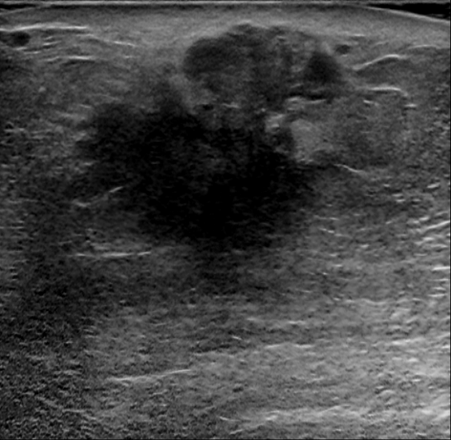
\includegraphics[trim=0 6 0 0,clip,height=.65\textheight]{a110105_094.png}~
\end{frame}

\begin{frame}[plain]\frametitle{Breast Lesion Segmentation in US images}
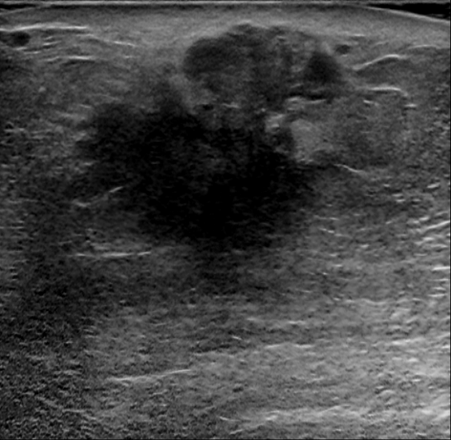
\includegraphics[trim=0 6 0 0,clip,height=.40\paperwidth]{a110105_094.png}~
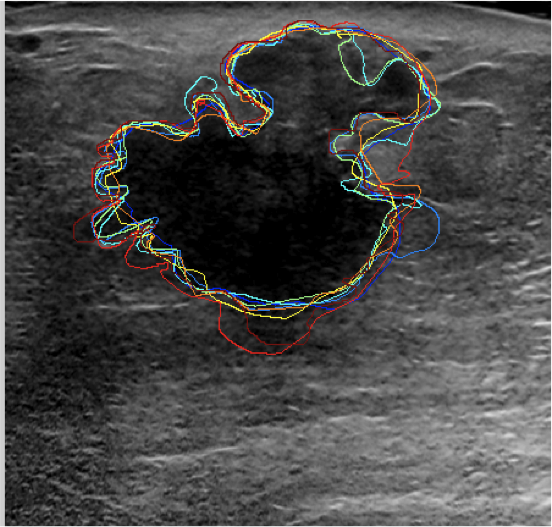
\includegraphics[trim=6 0 0 0,clip,height=.40\paperwidth]{segment.png}
\end{frame}

